\Chapter{Az alkalmazás tervei, megvalósítása}

\Section{Képernyő szerkezet}

\SubSection{Tervek}

Kezdetben összeállítottam egy tervet, arra, hogy nagyvonalakban hogyan is képzelem el a játék felületének felépítését, kinézetét. Ezen a kezdetleges rajzon elhelyeztem a kártyapaklikat, a kártyákat az azokon szereplő értékekkel, a zsetonokat és egy zsetongyűjtő panelt is. Az alapvető elképzeléseim az alapján születtek meg, hogy az alapjáték felépítése mind a fizikális, mind a digitális verzióban ehhez hasonló.

\begin{figure}[h]
\centering
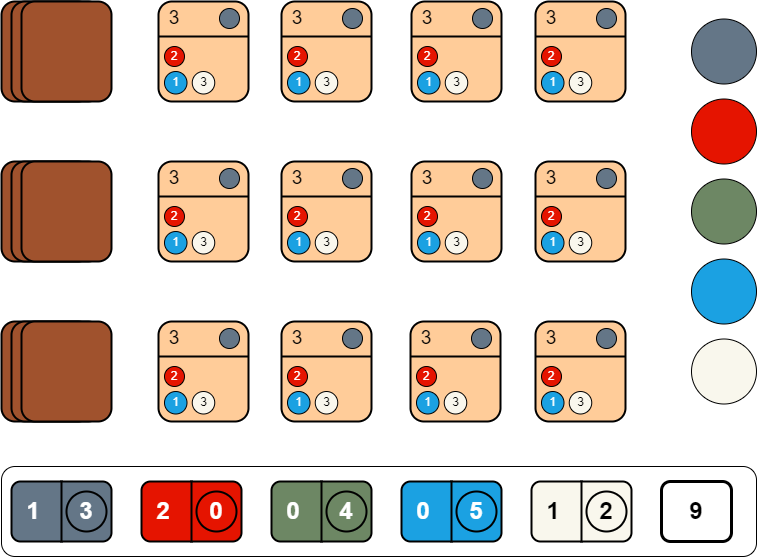
\includegraphics[scale=0.37]{images/screen_structure_plan.png}
\caption{A játék kezdetleges kinézeti terve.}
\label{fig:screen_structure_plan}
\end{figure}


\SubSection{Megvalósítás}

Az idő előrehaladtával formáltam mind a felépítést, mind a kinézetet, de a koncepció alapja megmaradt. A játék kapott egy hozzá illő hátteret, a kártyalapok színét is élőbbé tettem, a zsetonokat a halomban lévő számuk alapján megszámoztam és a zsetongyűjtő panelt is újraterveztem. Létrehoztam egy második panelt is a képernyő felső részén annak érdekében, hogy az adott játékos tudja követni az ellenfél részeredményeit is.
Emellett a jobb felső sarokba elhelyeztem egy "új játék" és egy "Játékszabályok" feliratú gombot, a hozzájuk tartozó funkciók ellátásához. Végezetül pedig megjelöltem a soron lévő játékost a hozzá tartozó panelének körberajzolásával és a játékost jellemző ikonnal.

\begin{figure}[h]
\centering
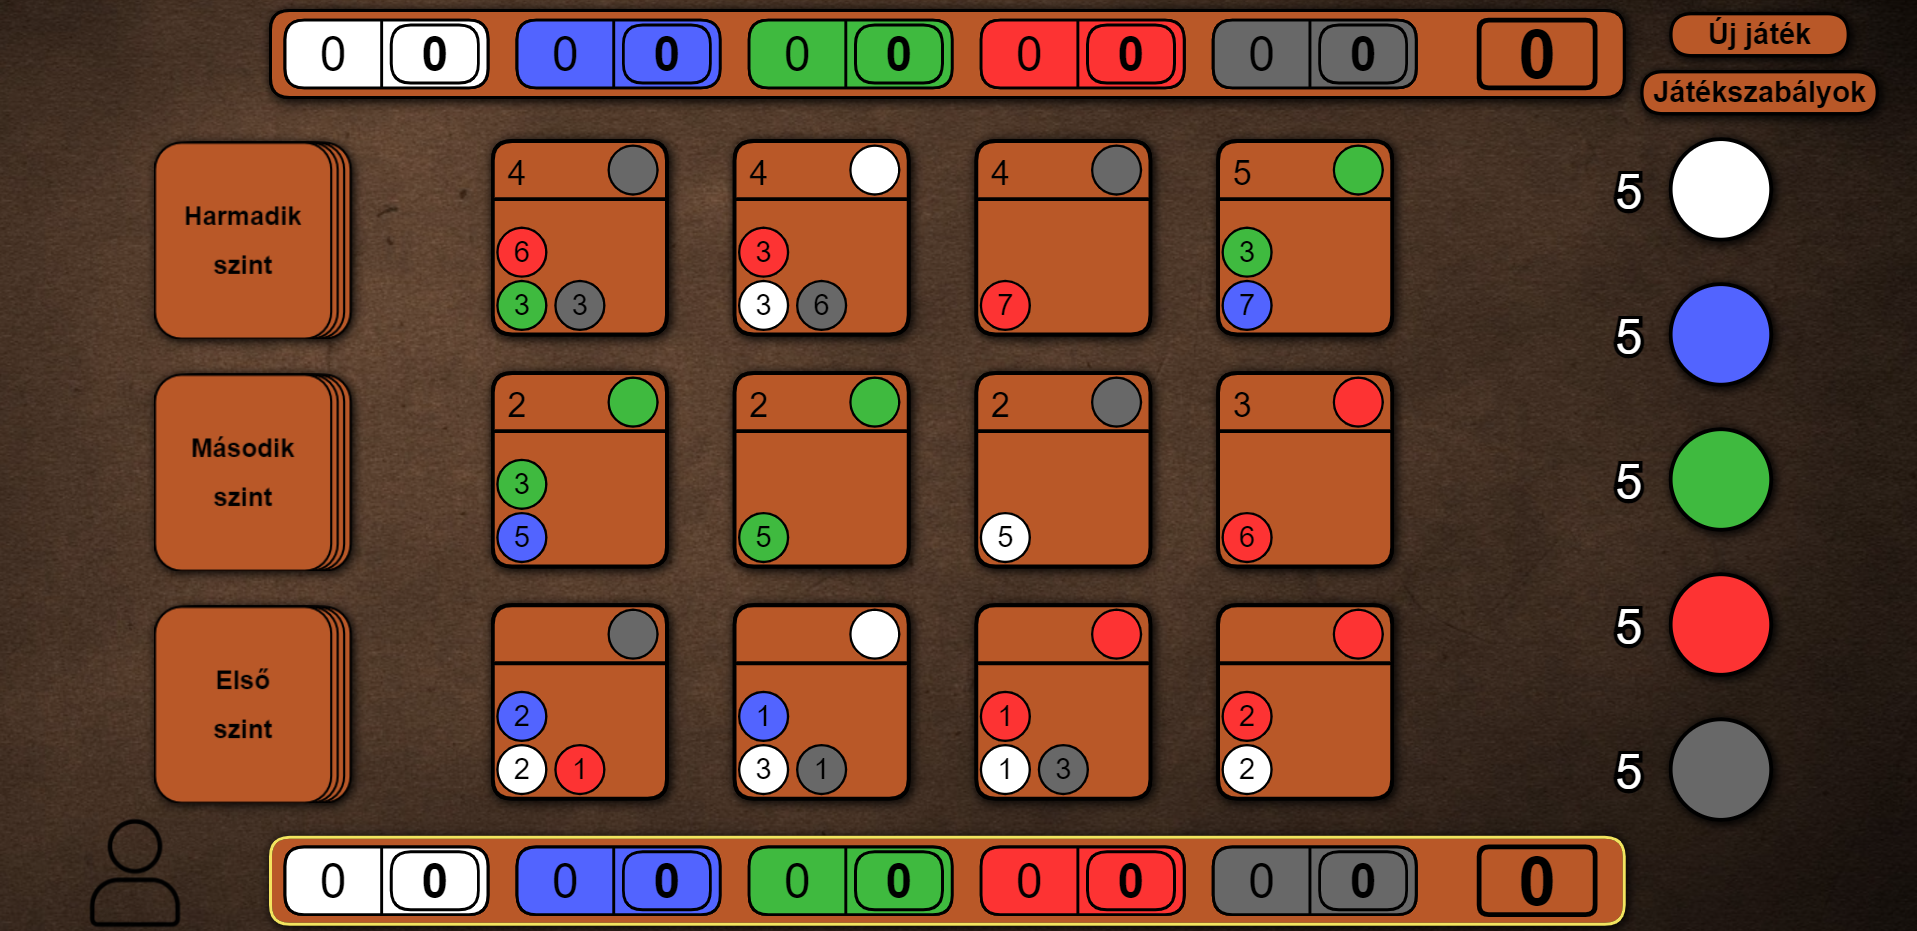
\includegraphics[width=\textwidth]{images/screen_structure.png}
\caption{A játék végleges kinézete.}
\label{fig:screen_structure}
\end{figure}

% TODO: Érdekes lehet ide egy kép a komponensek (osztályok) nevével.

\Section{Alapok}

Az általam leszűkített szabályrendszer alapú játék megvalósításához a JavaScriptet, a megjelenítéséhez pedig főleg a HTML5 Canvast, minimálisan pedig a CSS-t használtam.

\Section{Fáljrendszer kialakítása}

A játék fájlrendszerének alapját egy index nevű html fájl adja, amelyben magát a webes felület hoztam létre. Ide importáltam az összes szükséges JavaScript fájlt és beállítottam, hogy induláskor hívja meg a main.js fájlban meghatározott inicializáló függvényt. A main fájl gyűjti össze az összes funkciót, amit a játék magában foglal. Itt vannak definiálva a canvas alapfüggvényei, például a kattintás, egér mozgatás funkciók, valamint az imént említett inicializáló függvény, ami a canvast és a hozzá tartozó függvényeket érinti. A fájlok mellett van egy data nevű mappa, ahova a játék egész kártyakészletének adatait mentettem. Emellett egy classes nevű mappa is, ahol az objektumok és funkciók szerint szeparált JavaScript osztályok találhatóak. Végezetül pedig egy AI elnevezésű mappa, amelyekbe az általam fejlesztett számítógépes logikák fájljait helyeztem.


\Section{Kártyalapok}

A lapok körvonalát másodfokú görbék segítségével hoztam létre, az ezeken lévő zsetonokat pedig a megfelelő színnel kitöltött körrel valósítottam meg. A pontszámot és a bónusz zsetont jelölő kört egy vonallal választottam el a többi adattól. A pontszám a jobb, a bónusz pedig a bal felső sarkába került a kártyalapnak. A kártya alsó felén helyeztem el a megvásárláshoz szükséges zsetonokat az értékeikkel együtt, úgy, hogy a paraméterként megkapott értékektől függően balról jobbra, lentről felfelé töltődnek fel a pozícióik. Meghatároztam a játék során végig használt alapszínek RGB kódját is.

\Section{Zsetonok}

A zsetonokat körök kirajzolásának segítségével hoztam létre, amelyeket a megfelelő színnel töltöttem ki, és melléjük kiírattam az adott halomban lévő zsetonok számát.


\Section{Zsetongyűjtő panel}

Létrehoztam a panel elemek számára egy osztályt, ahol az adott elem kirajzolását valósítottam meg. A háttérszínét a hozzá tartozó színnel töltöttem ki, két részre osztottam egy függőleges vonallal és a bónusz értéket egy külön körvonallal jelöltem meg. Ezután létrehoztam a panelnek is egy külön osztályt, ahol inicializáltam a különböző panel elemeket, a panel jobb szélén pedig létrehoztam a pont számítására levő elemet. A panel és a panel elemek körvonalát szintén másodfokú görbék segítségével rajzoltam meg.

\Section{Tábla osztály}

A tábla osztályban terveztem összefogni a játék elemeit, és a játék kirajzolásának, működésének, szabályainak megvalósítását. Kezdetben a játék elemeinek elhelyezkedését szerettem volna meghatározni. Kitaláltam a kártyák megfelelő pozícióját és elhelyeztem őket sorban, egyelőre még csak véletlenszerűen az összes kártya közül kiválasztva, nem a megfelelő szintekre bontva. Ezután a panelek, a zsetonok és a kártyapaklik elhelyezése következett, még a megfelelő értékeik nélkül. Majd pedig beállítottam a táblának a hátterét is.

A következő szakaszban a már elhelyezett elemeknek az értékeire helyeztem a hangsúlyt. Igyekeztem a hozzájuk tartozó megfelelő értékeket társítani. Megvalósítottam, hogy a kártyák a szintjeik alapján legyenek kiválogatva külön tömbbe. Ezeket a tömböket megkevertem, majd ebből kihúztam és elhelyeztem a lapokat a játéktérre a játékszabály által leírt módon. A zsetongyűjtő panelre is a hozzá tartozó megfelelő értékeket írtam ki, és a zsetonoknak is megadtam a kezdő értéküket.

\Section{Egér mozgatás}

Ezután a kártyák és a zsetonok egér mozgatásra való interakcióját kezdtem el megvalósítani. Kezdetben egérkattintásra néztem meg, hogy a kártyákra és zsetonokra kattintva a megfelelő indexű és koordinátájú elemet kapom-e vissza. Azt, hogy az egér beleesik-e az adott kártya vagy zseton területébe a koordinátájukból, a magasságukból és a szélességükből kiszámítva határoztam meg. Kezdetben a tábla osztályban egy függvényben határoztam ezt meg, később viszont a kártya saját osztályában, önmaga dönti el, hogy éppen a kurzor alatt van-e vagy sem. Ezután a már működő programrészt átültettem az egér mozgatására és megjelöltem az egér alatt lévő elemet úgy, hogy a körvonalát egy világos, sárga színnel rajzoltam körbe. Emellett a kurzor típusát is átállítottam az esetben, amikor egy kártya vagy zseton felett van.

\Section{Interakciók}

A játékon belüli interakciókat a zsetonvásárlással és az ennek hatására történő panel értékek feltöltésével kezdtem. Ezt úgy valósítottam meg, hogy a korábban meghatározott egér kattintáskor kiszámolt zseton értéket megkapva, a megfelelő színű halmot csökkentettem, a panelen viszont növeltem ezt az értéket.

Ezután a kártyavásárlással járó történésekkel foglalkoztam. Kezdetben azt valósítottam meg, hogy kattintáskor a kurzor alatt található kártya eltűnjön, majd a helyére a megfelelő, megkevert részpakliból kerüljön a következő lap. A bónusz értékek megszerzését is feltüntettem a panelen. A birtokba vétel után, a kártyán található pontszám (amennyiben van) hozzáadódik a panelen található játékos pontszámához. A zsetonok a szabályok alapján olyan módon kerülnek vissza a halmokba, hogy ami felhasználásra került, azt mind vissza kell szolgáltatni a játéktérre, ami viszont bónusz, az a játékos birtokában marad. Amennyiben több zsetonnal rendelkezett a játékos az adott színből, mint amennyire a kártya megvásárlásakor szükség volt, a bónuszok közül az összes és a zsetonok közül a szükséges mennyiség kerül felhasználásra, így a többlet érték a játékosnál marad zseton formájában.


\Section{Szabályrendszer}

A szabályrendszer megalkotásának szempontjából a kártyák és a zsetonok elérhetősége jelenti az alapot, így ezek  lefektetésével kezdtem neki ennek a területnek.

A szabályok alapján akkor lehet megvásárolni egy kártyát, ha a játékos birtokában van a lapon feltüntetett zsetonszám a megadott színekből, akár zsetonokból, akár a korábban megszerzett bónuszokból kifizetve azt. Valamint fontos, hogy kártyavásárlás esetén mást nem csinálhat a körében és amennyiben felvett egy zsetont, visszafordítani nem tudja az eseményeket.

A zsetonok kiválasztása ennél egy fokkal bonyolultabb. Alapvetően egy zseton akkor elérhető a játékos számára, ha az adott halomban legalább egy található, ezen felül viszont a zsetonhúzás két féle módon tud történni egy kör során. Az első esetben a játékos három zsetont választ, amelyek közül mindegyik különböző színű, a második lehetőség pedig, hogy két azonos színű zsetont választ, de ezt csak abban az esetben tudja megtenni, ha az adott halomban a kör elején legalább négy zseton található.

Ezeknek a feltételrendszereknek a megvalósítása külön függvényekben történik, amelyeket a kártyára vagy a zsetonra való kattintáskor ellenőriz a program, hogy elérhető-e az adott játékos számára. Fontos, hogy az egy körön belül lévő korábbi cselekvéseink is korlátozhatják a lehetőségeinket, tehát ha zsetont vesz fel a játékos az első cselekvésekor, a kártyaválasztás már nem elérhető a számára. A zsetonok között is fellelhető ez a jelenség, például amikor kiválasztunk két különböző színű zsetont, azok már biztosan nem elérhetőek az adott körben, akármennyi is van a halomban, hiszen csak a három eltérő színű zsetonválasztás típusú lépéssorozat folytatható. Ezen felül a korábbi körök lépései is befolyásolják és akár korlátozzák a lehetőségeinket. Amikor a kör kezdetén egy három zsetont tartalmazó halomból húzunk fel egyet, az már továbbra nem elérhető számunkra a kör során, mivel kettő felhúzása nem lehetséges a zsetonszám miatt. Továbbá a kifogyott halmok sem elérhetőek a játékosok számára, így akár felmerülhet olyan esemény, amikor a három különböző színű zseton felvételekor nem elérhető a maximális számú lehetőség, így csak annyit vehetünk fel, amennyi a rendelkezésünkre áll a szabályok szerint.

\Section{Körökre osztás}

A játékot az aktuális játékos indexe alapján bontottam körökre. Létrehoztam a játékos osztályt a megfelelő értékekkel és inicializáltam őket a tábla osztályon belül a többihez hasonlóan, összekapcsolva a hozzájuk tartozó panelekkel. Bevezettem a kattintások dokumentálására egy változót, amelyben eltároltam az éppen játékban lévő játékos a köre megkezdésétől megtett, a szabályok és a játék akkori állása alapján megengedett kattintásait. A kártya vásárlásakor az indexe, a zseton megvásárlásakor pedig a színe kerül bele. Ezen információk segítségével ítéli meg a program, hogy vége van-e az adott játékos körének. Amikor az első cselekvés kártyavásárlás volt, a kör azonnal átadódik a másik játékosnak. Ellenkező esetben figyeli a kattintások tömbjét. Amennyiben kettő azonos színű zseton lett kiválasztva, szintén a következő játékosra vált. Az utolsó lehetőség esetén pedig ellenőrzi, ha az első és a második választott zseton színe nem egyezik, akkor a harmadiknak sem szabad egyeznie egyikkel sem, miután pedig ez megfelelt a kritériumoknak a kör szintén a következő játékosé lesz.

\Section{Ablakátméretezés}

Az ablakátméretezés problémáját is meg szerettem volna oldani, hogy akármilyen ablakméretnél lehessen játszani a játékkal. Ezt az ablak koordinátáinak ellensúlyozásával, transzformálásával és skálázásával oldottam meg. Az alábbi képeken látható, hogy miként néz ki a játéktér különböző ablakméretek mellett.

\begin{figure}[h]
\centering
$\vcenter{\hbox{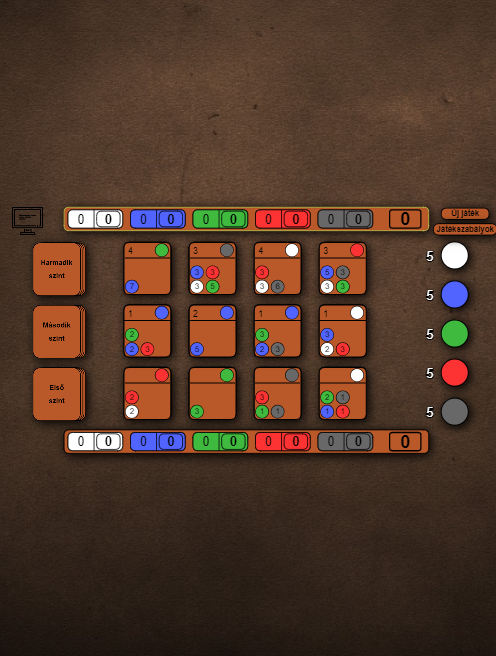
\includegraphics[scale=0.2]{images/resize1.png}}}$
\hspace{1cm}
$\vcenter{\hbox{
\includegraphics[scale=0.2]{images/resize2.png}}}$
\caption{A játék kinézete különböző ablakméret mellett.}
\label{fig:resize}
\end{figure}

\Section{Esztétikai beállítások}

A játéktéren található elemek formázását a Canvas segítségével, az ezen kívül található (például a kezdőképernyő, játék végén felugró felület, stb.) felületek formázását viszont CSS segítségével valósítottam meg. Azért követtem ezt a logikát, hiszen a játéktéren, a játékmenettel kapcsolatos dolgok összetartoznak és jó, ha egy logika alapján vannak formázva, míg az ezen kívüli elemek egy másik csoportot alkotnak, amelyeket egyszerűbbnek tartottam CSS-ben megvalósítani.

\SubSection{Játékos számára releváns információk}

Kiemeltem grafikusan a játékosok számára fontos információkat, ezáltal jobban átláthatóbbak a lehetőségek. Zöld színű, vékony vonallal körberajzoltam az elérhető kártyákat, az éppen nem elérhető zsetonoknak viszont szürke körvonalat adtam, így az egér mozgatására sem látható a kiválaszthatóságuk. Az éppen körön lévő játékos paneljét is egy vékony, sárga vonallal rajzoltam körbe, valamint a képernyő bal oldalán, az aktuális panel mellet megjelenítettem egy játékost jellemző ikont is, így egyértelműbbé válik, hogy melyik játékos van soron.

\SubSection{Kezdőképernyő}

Ezután megalkottam és megformáztam a kezdőképernyőt, ami minden játékindításkor megjelenik a felhasználó számára. Ennek a felületnek az alapja a játék táblájának elhomályosítása, amelyen egy kiírás és két gomb található. A felirat felszólítja a játékost, hogy válassza ki az adott játékban szereplő játékosokat. A két gomb a két lehetőséget reprezentálja, miszerint vagy két emberi, vagy pedig egy emberi és egy számítógép által vezérelt játékos fog játszani. Ezeknek a megjelenítését és az eseménykezelését CSS segítségével valósítottam meg.


\SubSection{Gomb interakciók}

Ez követően a játéktéren található gombokkal foglalatoskodtam, amelyeknek létrehoztam egy külön osztályt a megfelelő paramétereikkel, tehát ezeket a gombokat az előzőkkel ellentétben a Canvas segítségével valósítottam meg. Először csináltam egy "Új játék" feliratú gombot, amellyel a játék során akármikor új játékot lehet kezdeni. Ezt követően pedig a hasonló felépítésű "Játékszabályok" elnevezésű gombot helyeztem el a képernyőn, amelyre való kattintással egy olyan felület jön elő, ahol a játékszabályokat olvashatjuk el. Ez a felugró felület CSS-ben lett megalkotva. Az alap szintén az elhomályosított tábla, amelyen egy kerettel és háttérrel rendelkező felirat doboz helyezkedik el. Ezen a felületen található az általam megvalósított játékverzió szabályai. Ebből a felületből való kilépést az elhomályosított területre való kattintással valósítottam meg. A tábla elemekhez hasonlóan a kurzor mozgatásra reagáló megjelenést hoztam létre a gombok számára is, miszerint a betűszínük sárgával van átrajzolva, amennyiben az egér alatt találhatók.


\SubSection{Elérhető lépések megszűnése}

Ahogy korábban is említettem, a játékszabályok módosításával sajnos felmerülhet egy olyan játékállapot, amikor az adott játékos sem kártyát, sem zsetont nem tud választani. Ezt az eshetőséget a korábbiakhoz hasonlóan olyan formában orvosoltam, hogy a jelenség bekövetkezésekor megjelenik egy szöveg, amely tájékoztatja a játékost a felmerült problémáról, és arról, hogy ennek az üzenetnek a bezárása után újraindul a játék.

\newpage

\SubSection{Záró képernyő}

A játék végét jelentő feltételt követően pedig megjelenik a záró képernyő, amelyen látható egy felirat és egy gomb. A szöveg tájékoztatja a felhasználót arról, hogy melyik játékos nyerte a játékot, a gomb pedig lehetőséget ad a játék újrakezdésére, amely megnyomásával megjelenik a kezdőképernyő. Ezt a felületet a kezdőképernyőhöz hasonlóan formáztam meg mind a hátteret, mind a feliratot, mind a gombot tekintve.

\SubSection{Esztétika és refaktorálás}

A játék fejlesztésének egészében folyamatosan zajlottak a kódrészek átszervezései, refaktorálása, egyszerűbbé, egyértelműbbé tétele, valamint az esztétikai fejlesztések, javítgatások. Ahogy viszont többek között a tábla osztályon is észrevehető, ezek a folyamatok azonban nincsenek maradéktalanul elvégezve, ami a program szempontjából a megvalósított játékszabályok és funkciók bővítése mellett továbbfejlesztési lehetőségek.

\Section{Osztálydiagram}

\begin{figure}[h]
\centering
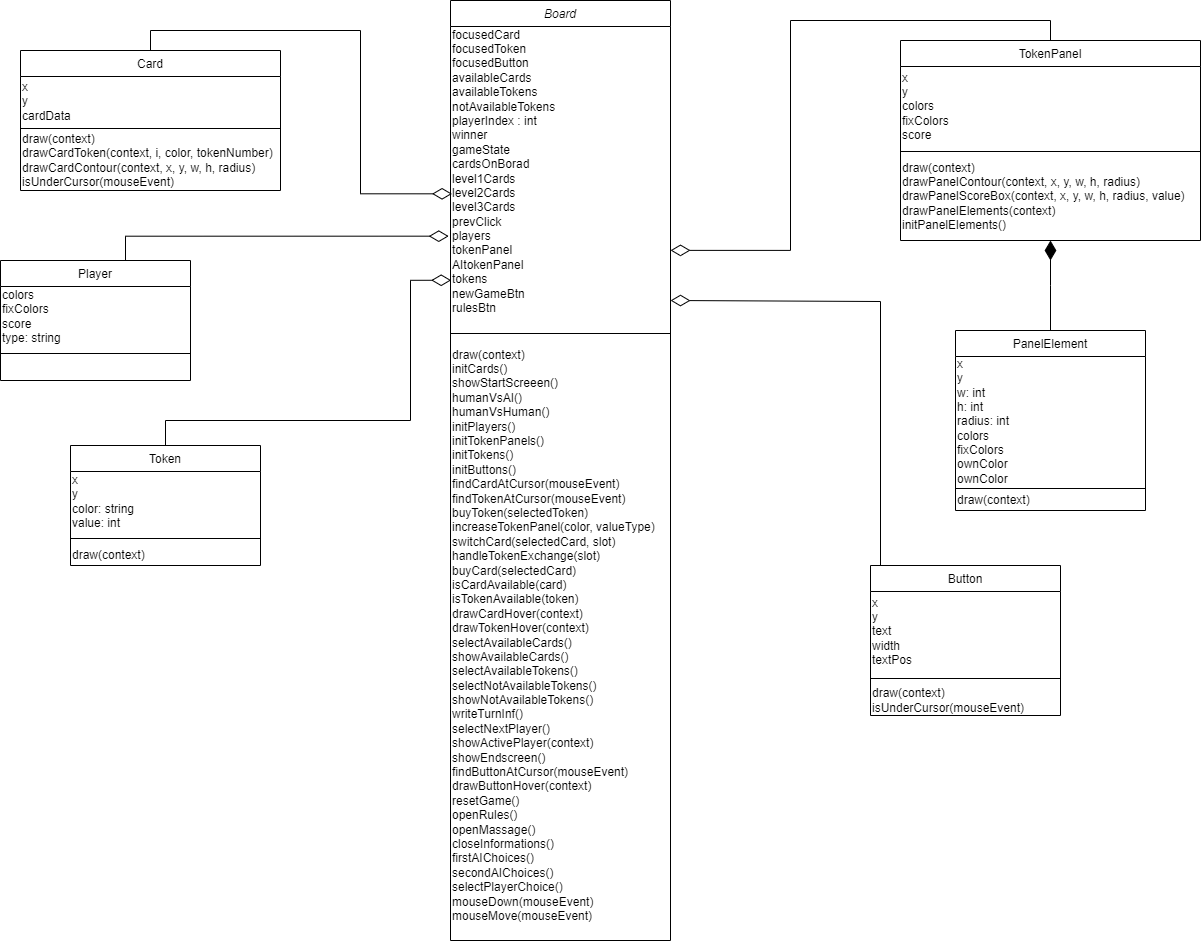
\includegraphics[scale=0.35]{images/UML.png}
\caption{A játék megvalósításának osztálydiagramja.}
\label{fig:uml}
\end{figure}

% TODO: Érdekes lenne majd bemutatni, hogy refaktorálást követően hogy lennének az osztályok.

